\newpage
\section{ioFog}
ioFog is an edge computing platform for deploying, running, and networking distributed microservices at the edge. It is a management platform for managing microservices/applications on edge nodes \cite{ioFogCoreConcepts}. This is very similar to running microservices in a Kubernetes cluster, except in ioFog you have a very granular control of microservice deployment to selected agents. Microservices are packed inside container images and get then executed on the Docker container runtime \cite{ioFogArchitecture}. Figure \ref{fig:iofog-ecn-architecture} shows a basic architecture consisting of one control plane and two agents.

\begin{figure}[H]
    \centering
    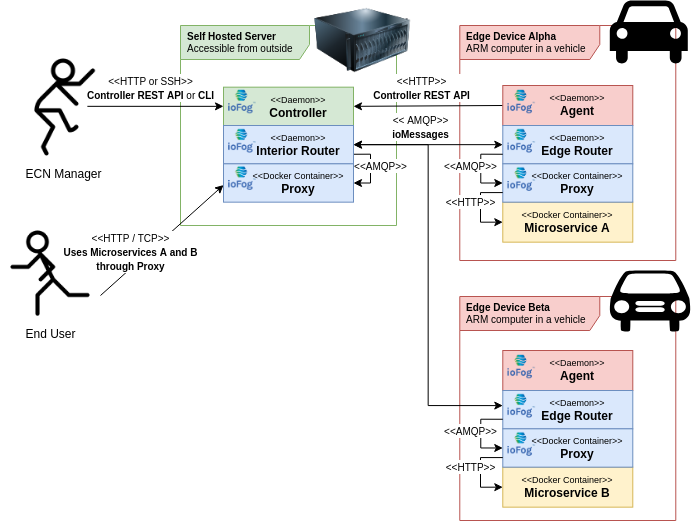
\includegraphics[width=\textwidth]{assets/iofog/iofog-architecture-ecn-router.png}
    \caption{ioFog Architecture \cite{ioFogArchitecture}.}\label{fig:iofog-ecn-architecture}
\end{figure}


\paragraph{Controller:} The controller is the master node of the \gls{ECN}. It orchestrates all agents, applications, microservices, and much more. The only requirement for the controller is the accessibility to it. Each agent, in the \gls{ECN}, needs access to the controller to get its instructions. A common solution is to deploy the controller to a cloud provider like \gls{AWS}, Microsoft Azure or Google Cloud Platform as the documentation suggests, but a local installation is also a viable solution. One node cannot contain both a controller and an agent daemon \cite{ioFogArchitecture}.

\paragraph{Agent:} The agent is the worker unit of the \gls{ECN}. Agents are typically deployed on the edge, e.g. near sensors, as native daemons. Each agent has the capability for running microservices, mounting volumes and managing resources. Microservices are represented as docker containers. An agent has not to be accessible from the outside, it only needs a connection to the controller. The agent receives instructions from the controller and also reports about its status \cite{ioFogArchitecture}.

\paragraph{Microservices:} Microservices are applications packed as Docker containers. Microservices get executed on the agent's Docker daemon \cite{ioFogArchitecture}.

\paragraph{Router:} The ioFog Router is an essential component that connects microservices together for communicating with the integrated messaging solution ioMessages. It also enables public port tunneling to microservices \cite{ioFogArchitecture}.

\paragraph{Proxy:} The Proxy is a microservice running on each agent. Its purpose is to translate HTTP requests to AMQP which is used by the routers as communication protocol \cite{ioFogArchitecture}.


\subsection{Use case implementation}
Figure \ref{fig:ioFog-arch} shows a simplified overview about the architecture built with the edge computing platform ioFog. Each yellow rectangle represents one agent of ioFog. The gray rectangle is the node with the control plane. Blue rectangles represent the on the node running docker engine.

\begin{figure}[H]
    \fontsize{6}{10}\selectfont
    \centering
    \def\svgwidth{\textwidth}
    \input{assets/iofog/iofog-arch-overview.drawio.pdf_tex}
    \caption{ioFog architecture overview.}\label{fig:ioFog-arch}
\end{figure}


\subsubsection*{Node setup}
All three nodes and the fourth node, which was added later, were provisioned with the \textit{iofogctl} command line tool. This tool is provided alongside ioFog to create and manage an ioFog \gls{ECN}. To provision a control plane or an agent, the command line tool requires the input of an YAML configuration file. This YAML file contains all information about the node itself and how to connect to it. Listing \ref{lst:ioFog-master-config} and listing \ref{lst:ioFog-agent-config} shows the entire configuration file used to provision the first control plane and the first agent. More configuration options can be found at the control plane and agent configuration YAML specification\footnote{\url{https://iofog.org/docs/2/reference-iofogctl/reference-control-plane.html}} \footnote{\url{https://iofog.org/docs/2/reference-iofogctl/reference-agent.html}}. Unlike the AWS Greengrass core installer, the \textit{iofogctl} command line tool installs all the required packages, like docker, on each node.

\bigskip
As the \gls{ECN} architecture figure \ref{fig:iofog-ecn-architecture} shows there two types of nodes, the control plane and the agents. The node with the control plane cannot contain an agent, therefore this setup includes one control plane and two agents respectively later three agents.

\noindent\begin{minipage}{.45\textwidth}
\begin{lstlisting}[caption={Control plane provisioning configuration.},label={lst:ioFog-master-config}]
---
apiVersion: iofog.org/v2
kind: ControlPlane
metadata:
  name: master
spec:
  controllers:
  - name: master-1
    host: 192.168.178.150
    ssh:
      user: ubuntu
      keyFile: ./keys/id_rsa
\end{lstlisting}
\end{minipage}\hfill
\begin{minipage}{.45\textwidth}
\begin{lstlisting}[caption={Agent one provisioning configuration.},label={lst:ioFog-agent-config}]
---
apiVersion: iofog.org/v2
kind: Agent
metadata:
  name: agent-1
  latitude: 46.204391
  longitude: 6.143158
spec:
  host: 192.168.178.151
  ssh:
    user: ubuntu
    keyFile: ./keys/id_rsa
\end{lstlisting}
\end{minipage}


\subsubsection*{Client devices}
The same implementation for the k3s client devices from subsection \ref{subsubsec:k3s-client-devices} can be used to connect to the MQTT broker on each agent. The only change which has to be made is the direct connection to one of the agents due to the missing load balancer, each client device is tied to exactly one agent.

\subsubsection*{MQTT}
The edge computing platform ioFog does not come with a built-in MQTT broker. Therefore, a MQTT broker was deployed as a ioFog application. The used MQTT broker, EMQX, is the same as the one in the k3s (\ref{subsubsec:k3s-mqtt}) example with one difference. Unlike the k3s MQTT brokers, the MQTT broker for each ioFog agent operates on a standalone basis and is therefore not in cluster mode. By exposing the ports of the broker client, like shown in listing \ref{lst:ioFog-mqtt-config} on line 73, devices can connect to the agent by using its IP address.

\begin{lstlisting}[caption={Example MQTT microservice configuration.},label={lst:ioFog-mqtt-config},captionpos=b]
apiVersion: iofog.org/v2
kind: Application
metadata:
  name: mqtt
spec:
  microservices:
    - name: mqtt-1
      agent:
        name: agent-1
      images:
        arm: docker.io/emqx/emqx:4.2.14
        registry: remote
      container:
        ports:
          - internal: 1883
            external: 1883 # <-- exposing MQTT port to the outside
    ...
\end{lstlisting}

One problem which occurs with this MQTT broker and the service on the same agent which want to subscribe to topics of the broker is that there is no possibility to directly connect to the MQTT broker. The \gls{MQTT} broker and any other application on the agent do not share the same network namespace, hence no direct connection can be established. Also, the ability to directly connect inside the Docker created network is not possible due to the container naming convention. The only way to connect to the MQTT broker is to connect over the agent's IPv4 address.


\subsubsection*{Detector service}
For ioFog the application from the k3s (\ref{subsubsec:k3s-detector}) example can be reused. Unlike in the k3s (\ref{subsubsec:k3s-detector}) example there is no need for specific selection of a node due to the fact that ioFog microservices are always specifically targeted to one agent only. The agent selection is always done by setting the agent name on the \textit{"agent.name"} attribute inside the YAML configuration. The agent selection is shown in listing \ref{lst:ioFog-detector-config} on line 6. Besides the agent selection, the \gls{usb} devices needs to be mounted into the container by attaching it as a volume like the listing \ref{lst:ioFog-detector-config} shows on the lines 12 to 15. Mounting the \gls{usb} device into the container requires the container to run in privileged mode, which is done by setting the \textit{rootHostAccess} attribute to \textit{true}, which is also shown in listing \ref{lst:ioFog-detector-config}.

\begin{lstlisting}[caption={Example detector microservice configuration.},label={lst:ioFog-detector-config},captionpos=b]
...
spec:
  microservices:
    - name: detector
      agent:
        name: agent-1
      images:
        arm: <detector-image>:<tag>
        registry: local
      container:
        rootHostAccess: true
        volumes:
          - hostDestination: /dev/bus/usb
            containerDestination: /dev/bus/usb
            accessMode: 'rw'
...
\end{lstlisting}

\subsubsection*{Emergency service}
Also the k3s emergency (\ref{subsubsec:k3s-detector}) version can be reused for ioFog. The service gets deployed on each of the agents and represents a standalone working unit. 

\subsubsection*{Database service}
Like \gls{AWS} Greengrass, ioFog is a more intermediary entity for the processing of data and not for the storage of such data. Therefore, no database is deployed on the agents. Sending results over the control plane to e.g. a Kubernetes cluster is an intended and viable solution. For the following section about the monitoring service, a InfluxDB was deployed to agent one.

\subsubsection*{Monitoring service}
A collection of services which represent the monitoring from subsection \ref{subsec:monitoring-service}. This collection includes the Telegraf\footnote{\url{https://www.influxdata.com/time-series-platform/telegraf/}} state metrics collector microservice, the time series database InfluxDB\footnote{\url{https://www.influxdata.com/}} and Grafana\footnote{\url{https://grafana.com/}} as visualization dashboard. The Grafana dashboard and the time series database are only deployed to a single agent (agent-1). The Telegraf microservice is deployed to both agents. Telegraf then collects metrics from the agent and the MQTT broker. The collected data will then be sent to the time series database on agent-1, which can be fetched from Grafana later on for visualization. To reach the Grafana dashboard from everywhere, its port is tunneled to the controller. By collecting all this data similar results like in the k3s figure \ref{fig:k3s-grafana-k3s-metrics} can be achieved.
